\documentclass[
size=17pt,
paper=smartboard,
mode=present,
display=slidesnotes,
style=paintings,
nopagebreaks,
blackslide,
fleqn]{powerdot}

% styles: sailor, paintings
% wj capsules prettybox
% mode = handout or present


\newcommand{\palette}{PearlEarring}
% palettes:
%    - sailor: Sea, River, Wine, Chocolate, Cocktail 
%    - paintings: Syndics, Skater, GoldenGate, Moitessier, PearlEarring, Lamentation, HolyWood, Europa, MayThird, Charon 


\usepackage{amsmath,graphicx,color,amsfonts}
\usepackage[brazilian]{babel}
\usepackage[utf8]{inputenc}
\usepackage{bbding}

\newcommand{\cursopequeno}{TC01001 FET}
\newcommand{\cursogrande}{\Large TC01001 -- Funções especiais em telecomunicações}
\newcommand{\alert}[1]{\textcolor{red}{#1}}
\newtheorem{theorem}{Teorema}
\author{Ronaldo de Freitas Zampolo\\FCT-ITEC-UFPA}
\date{2022-2}


\pdsetup{
   lf = {\cursopequeno},
   rf = {Série de Fourier}, palette = {\palette}, randomdots={false},
   cf = {\theslide}
}

\title{\cursogrande\\ \vspace{1cm}Série de Fourier}

\begin{document}
   \maketitle[randomdots={false}]
   \begin{slide}{Agenda}
      \tableofcontents[content=sections]
   \end{slide}

   \section[ slide = true ]{Introdução}
      \begin{slide}[toc=]{Introdução}
         	\twocolumn{
		\begin{itemize}
			\item Jean Baptiste Joseph Fourier 
				\begin{itemize}
					\item[\FiveStarShadow] 21/03/1768, Auxerre
					\item[\CrossOpenShadow] 16/05/1830, Paris
				\end{itemize}
			\item Matemático e físico
			\item 1822: \emph{Théorie Analytique de la Chaleur}
		\end{itemize}
		\begin{center}
			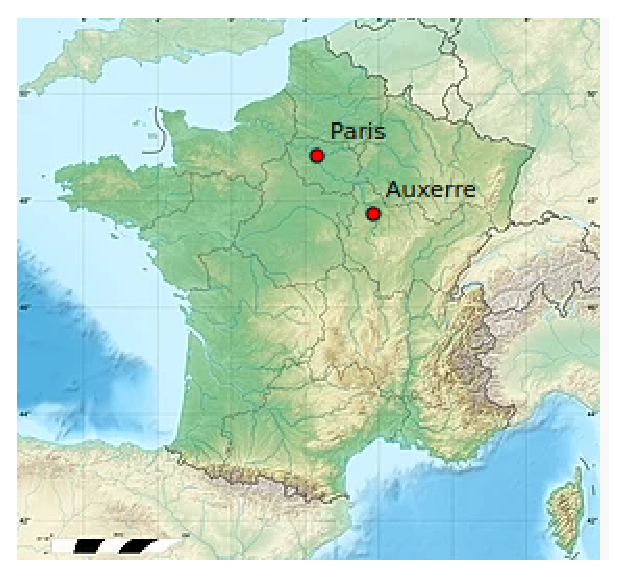
\includegraphics[width=0.65\textwidth]{figs/auxerre-paris}
		\end{center}
		}
		{
			\includegraphics[width=0.45\textwidth]{figs/Fourier2}%\pause
		%\begin{center}
	%		\includegraphics[width=0.7\textwidth]{figs/tombe-2015}
	%	\end{center}
		}
      \end{slide}

      \begin{slide}[toc =]{Introdução}
	      \begin{itemize}
		      \item Ideia básica: qualquer função $f(x)$ periódica em $2\pi$ pode ser representada por uma série trigonométrica infinita na forma
			      \begin{equation*}
				      f(x) = \frac{a_0}{2}+ \sum_{n=1}^\infty \left [ a_n\cos nx + b_n\sin nx\right ]
			      \end{equation*}\pause	
		      \item Objetivo inicial: resolução de equações diferenciais\pause
		      \item Atualmente é ferramenta essencial para análise de formas de onda\pause
		      \item Algumas áreas em que a análise de Fourier tem grande aplicação:
			      \begin{itemize}
				      \item Processamento de sinais
				      \item Análise de circuitos
				      \item Sistemas de controle
				      \item Telecomunicações
			      \end{itemize}
	      \end{itemize}
      \end{slide}
      
   \section[ slide = true ]{Série de Fourier de funções com periodicidade 2$\pi$}
      \begin{slide}[toc=]{Ortogonalidade de funções trigonométricas}
         \begin{itemize}
		 \item Condição de ortogonalidade de funções \alert{(compare com o produto escalar)}
		    \begin{equation*}
			    \int_a^b \psi_n(x)\psi_m(x) dx = 0,\quad  n\neq m
		    \end{equation*}
			 As funções $\psi_n$ e $\psi_m$ são ditas ortogonais no intervalo entre $a$ e $b$.\\ \pause
		 \item Considerando que $m\in \mathbb{Z}$ e $n\in \mathbb{Z}$, \alert{(convém deduzir, estudante)}
			 \twocolumn{
				 \begin{align*}
					 \int_{-\pi}^\pi \cos mx dx &= 0\qquad m\neq 0\\
					 \int_{-\pi}^\pi \sin mx dx &= 0\\
					 \int_{-\pi}^\pi \cos mx \sin nx dx &= 0\\
				 \end{align*}
				 }{
				 \begin{align*}
					\int_{-\pi}^\pi \cos mx \cos nx dx &= \begin{cases} 0 \quad m \neq n \\ \pi \quad m=n\neq 0\\2\pi \quad m=n=0\end{cases}\\
					\int_{-\pi}^\pi \sin mx \sin nx dx &= \begin{cases} 0 \quad m \neq n \\ \pi \quad m=n\neq 0\end{cases}
				 \end{align*}
				 }\pause
		\item Logo, as funções $1, \cos x, \sin x, \cos 2x, \sin 2x, \dots$ formam um conjunto ortogonal no intervalo entre $-\pi$ e $\pi$.
	\end{itemize}         
      \end{slide}
      
      \begin{slide}[toc=]{Determinação dos coeficientes de Fourier}
	      \begin{itemize}
		      \item Série de Fourier:
			      \begin{equation*}
				      f(x) = \frac{a_0}{2}+ \sum_{n=1}^\infty \left [ a_n\cos nx  + b_n\sin nx \right ]
			      \end{equation*}\pause	
		      \item Função periódica: $f(x+2\pi) = f(x)$\pause
		      \item Procedimento para determinação dos coeficientes $a_n$:\pause
			      \begin{itemize}
				      \item Multiplica $f(x)$ por $\cos mx$\pause
					      \begin{equation*}
						      f(x)\cos mx = \frac{a_0}{2}\cos mx+ \sum_{n=1}^\infty \left [ a_n\cos nx\cos mx  + b_n\sin nx\cos mx \right ]
					      \end{equation*}\pause	
				      \item Integra no intervalo de $-\pi$ a $\pi$\pause
					      \begin{equation*}
						      \int_{-\pi}^\pi f(x)\cos mx\, dx = \frac{a_0}{2}\int_{-\pi}^\pi\cos mx\, dx + \sum_{n=1}^\infty \left [a_n\int_{-\pi}^\pi \cos nx\cos mx\, dx + b_n\int_{-\pi}^\pi\sin nx\cos mx\, dx\right ]
					      \end{equation*}	
			      \end{itemize}
            \end{itemize}
      \end{slide}

     \begin{slide}[toc=]{Determinação dos coeficientes de Fourier}
	      \begin{itemize}
		      \item Procedimento para determinação dos coeficientes $a_n$ (cont.):
			      \begin{itemize}
				      \item Avalia as integrais resultantes
					      \begin{align*}
						      \int_{-\pi}^\pi f(x)\cos mx\, dx =& \frac{a_0}{2}\int_{-\pi}^\pi\cos mx\, dx + \\
						                                        &+\sum_{n=1}^\infty \left [a_n\int_{-\pi}^\pi \cos nx\cos mx\, dx + b_n\int_{-\pi}^\pi\sin nx\cos mx\, dx\right ]\\
						      =&\frac{a_0}{2}\int_{-\pi}^\pi\cos mx\, dx + \sum_{n=1}^\infty a_n\int_{-\pi}^\pi \cos nx\cos mx\, dx +\\
						      &+\sum_{n=1}^\infty b_n\int_{-\pi}^\pi \sin nx\cos mx\, dx
					      \end{align*}
			      \end{itemize}
            \end{itemize}
      \end{slide}

     \begin{slide}[toc=]{Determinação dos coeficientes de Fourier}
	      \begin{itemize}
		      \item Procedimento para determinação dos coeficientes $a_n$ (cont.):
			      \begin{itemize}
				      \item Avalia as integrais resultantes (cont.)
					      \begin{align*}
						      \int_{-\pi}^\pi f(x)\cos mx\, dx =&\frac{a_0}{2}\int_{-\pi}^\pi\cos mx\, dx + \sum_{n=1}^\infty a_n\int_{-\pi}^\pi \cos nx\cos mx\, dx +\\
						      &+\sum_{n=1}^\infty b_n\int_{-\pi}^\pi \sin nx\cos mx\, dx
					      \end{align*}\pause
					      \begin{align*}
						      \int_{-\pi}^\pi f(x)\cos mx\, dx =\begin{cases}
							      \frac{a_0}{2}\int_{-\pi}^\pi dx &= a_0\pi, \quad m=0\\
							      a_m\int_{-\pi}^\pi \cos mx\cos mx\, dx &= a_m\pi, \quad m>0
						      \end{cases}
					      \end{align*}\pause
				      \item Determina expressão para $a_n$
					      \begin{equation*}
						      a_n = \frac{1}{\pi}\int_{-\pi}^\pi f(x)\cos nx\, dx
					      \end{equation*}
			      \end{itemize}
            \end{itemize}
      \end{slide}

     \begin{slide}[toc=]{Determinação dos coeficientes de Fourier}
	      \begin{itemize}
		      \item Seguindo a procedimento semelhante, 
			      \begin{equation*}
				      b_n = \frac{1}{\pi}\int_{-\pi}^\pi f(x)\sin nx\, dx
			      \end{equation*}\pause
		      \item Resumo:
			      \begin{itemize}
				      \item Seja $f(x)$ uma função periódica com período $2\pi$, i.e., $f(x+2\pi) = f(x)$
				      \item Pode-se representar $f(x)$ por uma série trigonométrica do tipo
					      \begin{equation*}
						      f(x) = \frac{a_0}{2}+ \sum_{n=1}^\infty \left [ a_n\cos nx  + b_n\sin nx \right ]
					      \end{equation*}
				      \item Onde os coeficientes $a_n$ e $b_n$ são determinados pelas expressões
					      \begin{equation*}
						      a_n = \frac{1}{\pi}\int_{-\pi}^\pi f(x)\cos nx\, dx\qquad
						      b_n = \frac{1}{\pi}\int_{-\pi}^\pi f(x)\sin nx\, dx
					      \end{equation*}
			      \end{itemize}
            \end{itemize}
      \end{slide}

      \begin{slide}[toc=]{Expansão de funções em série de Fourier}
	      \begin{itemize}
		      \item Função quadrada periódica
			      \begin{equation*}
				      f(x) = \begin{cases}
					      -k  &-\pi < x < 0\\
					      k  &\quad 0 < x < \pi
					      \end{cases} \qquad \qquad f(x+2\pi) = f(x)
			      \end{equation*}
			      \begin{figure}
				      \centering
				      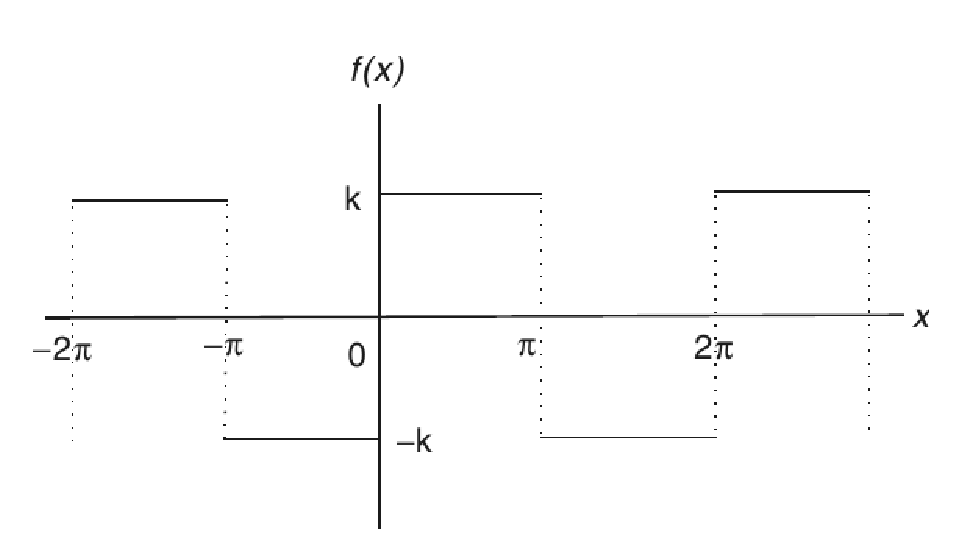
\includegraphics[width=0.5\textwidth]{figs/square-wave}
			      \end{figure}
	      \end{itemize}
      \end{slide}

      \begin{slide}[toc=]{Expansão de funções em série de Fourier}
	      \begin{itemize}
		      \item Determinação dos coeficientes de Fourier 
			      \twocolumn
			      {
				      \begin{align*}
					      a_0 &= \frac{1}{\pi}\int_{-\pi}^\pi f(x)\, dx\\
					      	  &= \frac{1}{\pi}\int_{-\pi}^0 (-k)\, dx + \frac{1}{\pi}\int_{0}^\pi k\, dx\\
						  &= 0
				      \end{align*}
				      \begin{align*}
					      a_n &= \frac{1}{\pi}\int_{-\pi}^\pi f(x)\cos nx\, dx\\
					      	  &= \frac{1}{\pi}\int_{-\pi}^0 (-k)\cos nx\, dx + \frac{1}{\pi}\int_{0}^\pi k\cos nx\, dx\\
						  &= 0
				      \end{align*}
			      }{
				      \begin{align*}
					      b_n =& \frac{1}{\pi}\int_{-\pi}^\pi f(x)\sin nx\, dx\\
					          =& \frac{1}{\pi}\int_{-\pi}^0 (-k)\sin nx\, dx + \\ 
						  &+\frac{1}{\pi}\int_{0}^\pi k\sin nx\, dx\\
						  =&\begin{cases}
							  \frac{4k}{n\pi}, & n\text{ é ímpar}\\
							  0, & n\text{ é par}
						  \end{cases}
				      \end{align*}
				}
	      \end{itemize}
      \end{slide}

      \begin{slide}[toc=]{Expansão de funções em série de Fourier}
	      \begin{itemize}
		      \item Representação usando série de Fourier
			      \begin{equation*}
				      f(x) = \frac{a_0}{2}+ \sum_{n=1}^\infty \left [ a_n\cos nx  + b_n\sin nx \right ]
					   =\sum_{n=1}^\infty \frac{4k}{\pi(2n-1)}\sin(2n-1)x
			      \end{equation*}
		      \item Serie truncada
			      \begin{equation*}
				      f_N(x)=\sum_{n=1}^N \frac{4k}{\pi(2n-1)}\sin(2n-1)x
			      \end{equation*}
	      \end{itemize}
      \end{slide}

      \begin{slide}[toc=]{Expansão de funções em série de Fourier}
	      Contribuição de cada componente espectral
	      \twocolumn{
		      \centering
		      $N=1$~~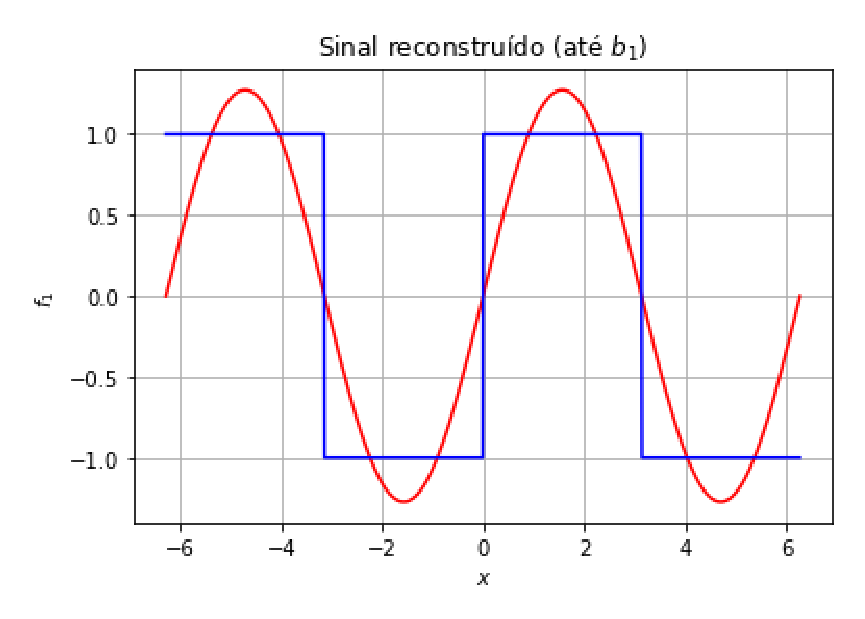
\includegraphics[width=0.5\textwidth]{figs/b1}
		      $N=2$~~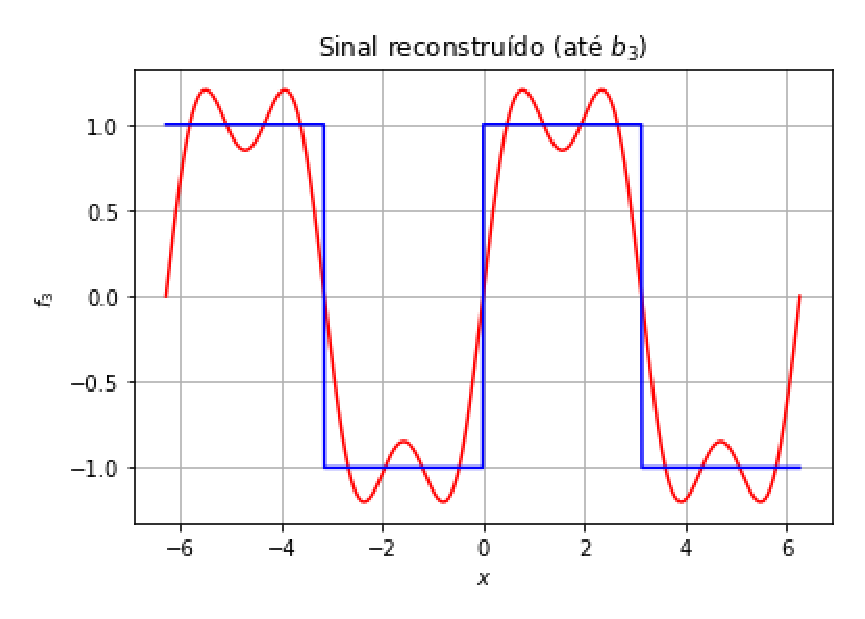
\includegraphics[width=0.5\textwidth]{figs/b3}
		      $N=3$~~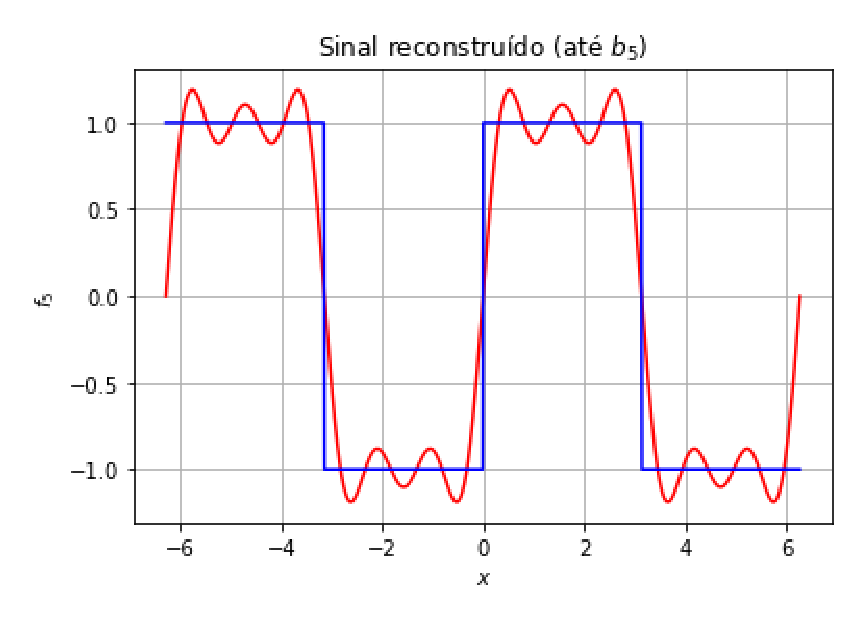
\includegraphics[width=0.5\textwidth]{figs/b5}
		      }{
		      \centering
		      $N=6$~~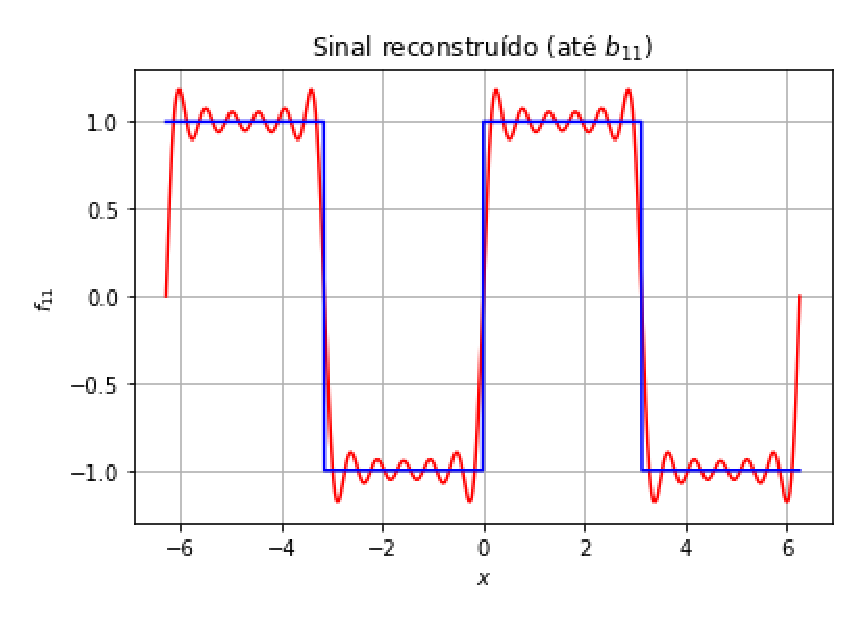
\includegraphics[width=0.5\textwidth]{figs/b11}
		      $N=26$~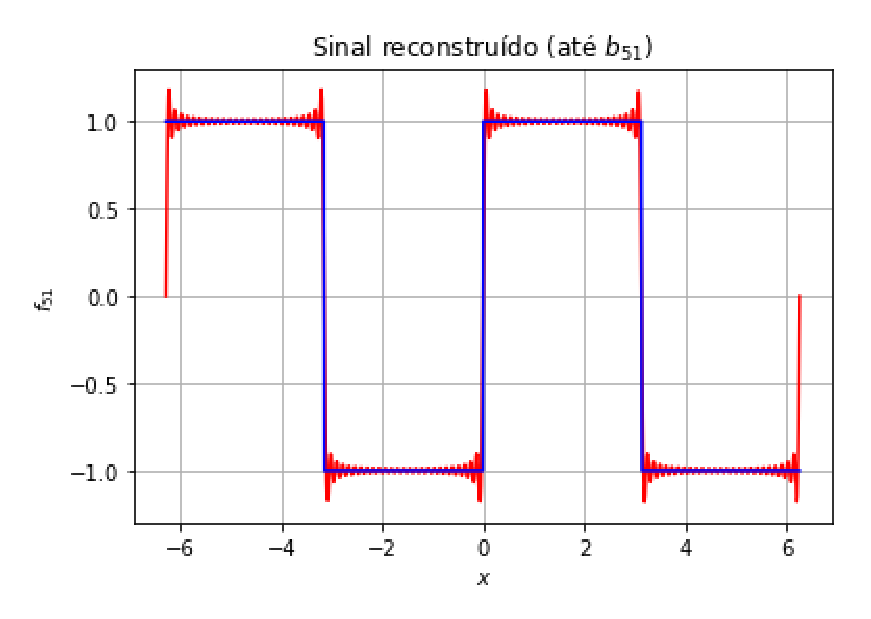
\includegraphics[width=0.5\textwidth]{figs/b51}
		      $N=50$~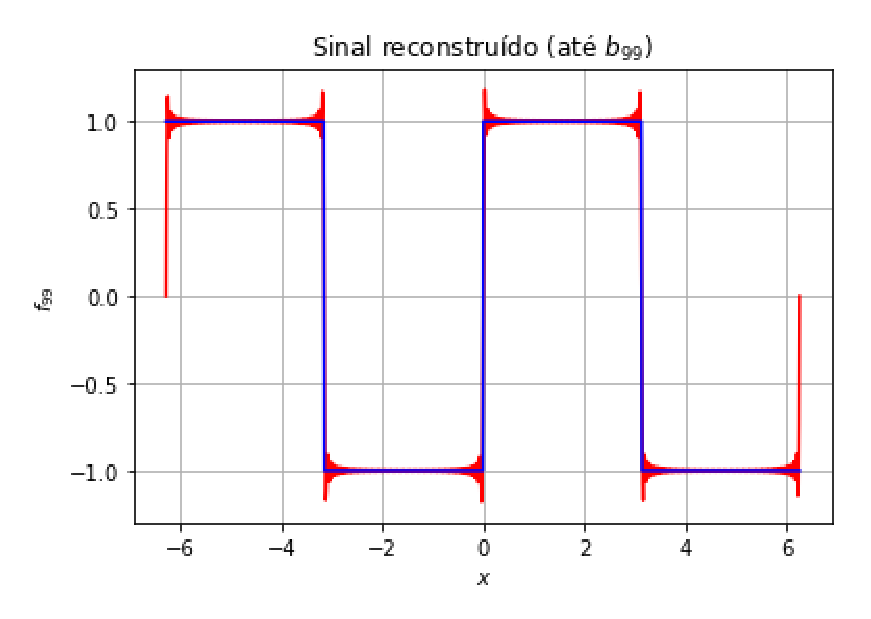
\includegraphics[width=0.5\textwidth]{figs/b99}
		      }
      \end{slide}

      \section[slide=true]{Convergência da série de Fourier}
      \begin{slide}[toc=]{Condições de Dirichlet}
	      \begin{theorem}
		      Se uma função periódica $f(x)$ de período $2\pi$ é limitada e contínua por partes, e tem um número finito de máximos e mínimos em cada período, então a série trigonométrica
			      \begin{equation*}
				      \frac{a_0}{2}+ \sum_{n=1}^\infty \left [ a_n\cos nx  + b_n\sin nx \right ]
			      \end{equation*}
		com 
					      \begin{align*}
						      a_n &= \frac{1}{\pi}\int_{-\pi}^\pi f(x)\cos nx\, dx & n=0,1,2,\dots\\
						      b_n &= \frac{1}{\pi}\int_{-\pi}^\pi f(x)\sin nx\, dx & n=1,2,3,\dots
					      \end{align*}
			converge para $f(x)$ onde $f(x)$ é contínua, e converge para a média dos limites à esquerda e à direita de $f(x)$ nos pontos de descontinuidade.
	      \end{theorem}
      \end{slide}
      
      \begin{slide}[toc=]{Condições de Dirichlet}
         \begin{itemize}
		 \item O teorema anterior estabelece \alert{condições suficientes} para convergência\pause
		 \item As condições mínimas necessárias para convergência não são conhecidas\pause
		 \item Pode-se assumir que \alert{todas as funções periódicas de interesse prático podem ser representadas pela série de Fourier}
         \end{itemize}
      \end{slide}

      %\begin{slide}[toc=]{Série de Fourier e função delta}
      %\end{slide}

      \section[ slide = true]{Série de Fourier de funções de período arbitrário}
      \begin{slide}[toc=]{Mudança de intervalo}
	      \twocolumn{
		      \begin{itemize}
			      \item A representação em série de Fourier pode ser generalizada para qualquer função periódica com período $2L$:
				      \begin{equation*}
					      f(t)=f(t+2L)
				      \end{equation*}
			      \item Para tanto, deve-se fazer a seguinte mudança de variável:
				      \begin{align*}
					      t    =& \frac{L}{\pi}x\\
					      f(t) =& f\left (\frac{L}{\pi}x\right )\equiv F(x)
				      \end{align*}
		      \end{itemize}
		 }
		 {\pause
		      \begin{itemize}
			      \item Dessa forma,
				      \begin{align*}
					      f(t)                           =& f(t+2L)\\
					      f\left (\frac{L}{\pi}x\right ) =& f\left (\frac{L}{\pi}x+2L\right )\\
					                                     =& f\left (\frac{Lx + 2L\pi}{\pi}\right ) \\
									     =& f\left (\frac{L}{\pi}(x+2\pi)\right )\\
						 F(x)                        =& F(x+2\pi)
				      \end{align*}\pause
			      \item Essa transformação de variável deve ser aplicada à série trigonométrica e às expressões para determinação de $a_n$ e $b_n$
		      \end{itemize}}
      \end{slide}
      
      \begin{slide}[toc=]{Mudança de intervalo}
	      Série trigonométrica:
	      \begin{equation*}
		      \frac{a_0}{2}+ \sum_{n=1}^\infty \left [ a_n\cos n\frac{\pi}{L}t  + b_n\sin n\frac{\pi}{L}t \right ]
	      \end{equation*}
	      Coeficientes de Fourier:
	      \begin{align*}
		      a_n &= \frac{1}{L}\int_{-L}^L f(t)\cos \left(n\frac{\pi}{L}t\right)\, dt & n=0,1,2,\dots\\
		      b_n &= \frac{1}{L}\int_{-L}^L f(t)\sin \left(n\frac{\pi}{L}t\right)\, dt & n=1,2,3,\dots
	      \end{align*}
	      Observações:
	      \begin{itemize}
		      \item $\pi/L$ é a frequência fundamental de $f(t)$
		      \item $n\pi/L$ é denominado harmônico de $f(t)$ (múltiplo da frequência fundamental)
	      \end{itemize}
      \end{slide}

      \begin{slide}[toc=]{Exercícios}
	      \begin{enumerate}
		      \item Sobre os exemplos 1.3.1, 1.3.2, e 1.3.3 no livro de referência: 
	      		\begin{itemize}
		      		\item Inicialmente, tentar resolver sozinho e, depois, comparar sua resolução com a apresentada no livro
		      		\item Aproximar as funções usando a série de Fourier truncada (aumente gradualmente o número de coeficientes usados) no Jupyter/Google Colab
		      		\item Observar a qualidade das reconstruções em função do número de coeficentes usados e das características das funções
	      		\end{itemize}
	      	   \item Repita exercício anterior para a função $f(t)$ periódica a seguir:
	      		\begin{align*}
		     		f(t)  =& \begin{cases}
			      		-t     & -1\leq t < 1\\
			      		t^2-4  &  1\leq t < 3\\
			      		-1     &  3\leq t < 4
		      		\end{cases}\\
		      		f(t) =& f(t+5)
	      		\end{align*}
	      \end{enumerate}
      \end{slide}

      \begin{slide}[toc=]{Série de Fourier de funções pares e ímpares}
	      \twocolumn{
		      \begin{itemize}
			      \item Função par
				      \begin{equation*}
					      f(t) = f(-t)
				      \end{equation*}
			      \item Função ímpar
				      \begin{equation*}
					      f(t) = -f(-t)
				      \end{equation*}
			      \item Produto entre funções:
				      \begin{itemize}
					      \item par $\times$ par, \alert{função par}
					      \item ímpar $\times$ ímpar, \alert{função par}
					      \item par $\times$ ímpar, \alert{função ímpar}
				      \end{itemize}
			      \item Sendo $g(t)$ uma \alert{função ímpar},
				      \begin{equation*}
					      \int_{-\epsilon}^\epsilon g(t) dt = 0
				      \end{equation*}
		      \end{itemize}
	      }
	      {
		      \begin{itemize}
			      \item Sendo $g(t)$ uma \alert{função par},
				      \begin{equation*}
					      \int_{-\epsilon}^\epsilon g(t) dt = 2\int_{0}^\epsilon g(t) dt
				      \end{equation*}
			      \item Se $f(t)$ for uma função par, 
				      \begin{equation*}
					      a_n = \frac{2}{L}\int_0^L f(t)\cos\left ( n\frac{\pi}{L}t\right )\, dt\qquad b_n = 0
				      \end{equation*}
			      \item Se $f(t)$ for uma função ímpar, 
				      \begin{equation*}
					      a_n = 0\qquad b_n=\frac{2}{L}\int_0^L f(t)\sin \left ( n\frac{\pi}{L}t\right )\, dt
				      \end{equation*}
		      \end{itemize}
	      }

      \end{slide}

      \section[ slide = true]{Série de Fourier de funções não-periódicas em faixa limitada}
      \begin{slide}{Representação de funções em faixa limitada}
	      \begin{itemize}
		      \item Ideia principal: usar série de Fourier para representar funções não periódicas em um determinado intervalo
		      \item Estratégia: considerar que fora do intervalo de interesse a função se repete, ou seja, é periódica
		      \item Estratégia melhorada: a partir da função original, formar funções periódicas pares (\emph{half-range cosine expansion}) ou ímpares (\emph{half-range sine expansion})
	      \end{itemize}
      \end{slide}
      
      \begin{slide}{Estratégia melhorada - exemplo}
	      \twocolumn
	      {
		      \begin{itemize}
			      \item Função original\\
				      \begin{center}
				      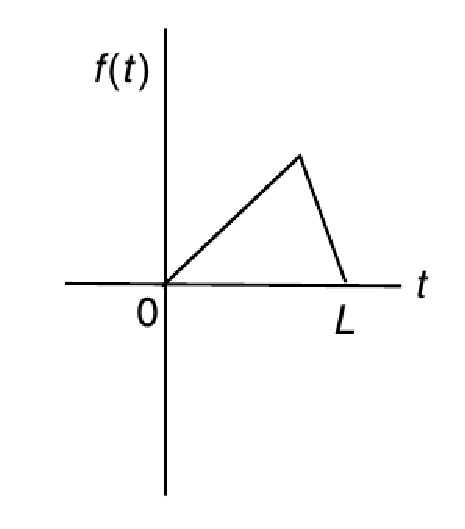
\includegraphics[width=0.7\textwidth]{figs/func}
				      \end{center}
		      \end{itemize}

	      }{
	      	      \begin{itemize}
	      		      \item Função extendida par\\
				      \begin{center}
				      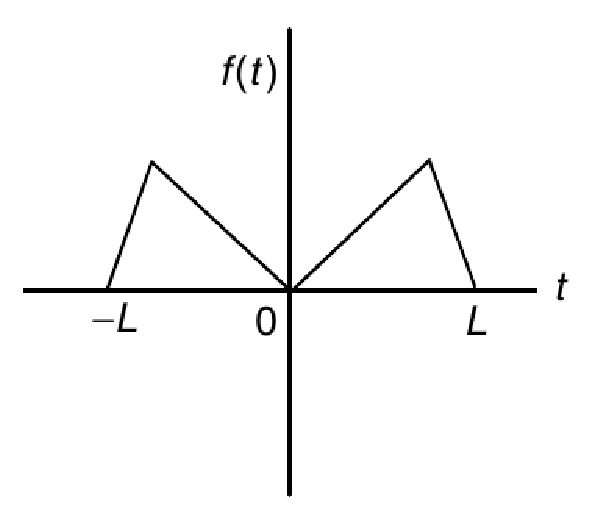
\includegraphics[width=0.5\textwidth]{figs/func-par}
				      \end{center}
			      \item Função extendida ímpar\\
				      \begin{center}
				      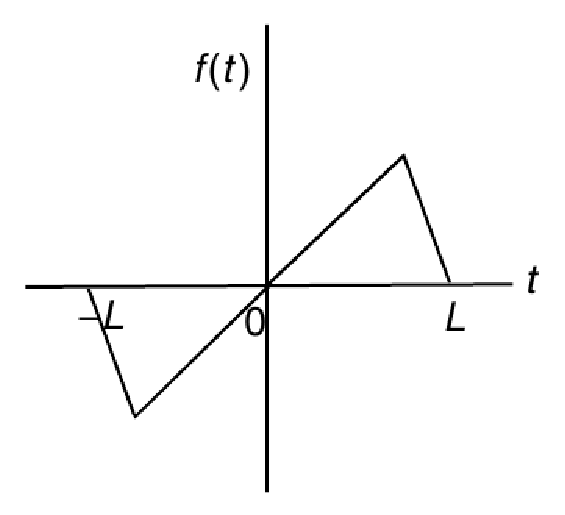
\includegraphics[width=0.5\textwidth]{figs/func-impar}
				      \end{center}
		      \end{itemize}
	      }
      \end{slide}

      \section[ slide = true]{Série de Fourier complexa}
      \begin{slide}{Série de Fourier complexa}
	      \twocolumn
	      {
	      Seja $f(t)$ expressa pela série trigonométrica
	      \begin{equation*}
		      f(t) = \frac{a_0}{2} + \sum_{n=1}^\infty \left [ a_n \cos \left ( n\frac{\pi}{L}t \right ) + b_n \sin \left ( n\frac{\pi}{L}t \right )\right ]
	      \end{equation*}
	      Usando a fórmula de Euler
	      \begin{align*}
		      \cos \left ( n\frac{\pi}{L}t \right ) =& \frac{e^{i\left ( n\frac{\pi}{L}t \right )} + e^{-i\left ( n\frac{\pi}{L}t \right )}}{2}\\ 
		      \sin \left ( n\frac{\pi}{L}t \right ) =& \frac{e^{i\left ( n\frac{\pi}{L}t \right )} - e^{-i\left ( n\frac{\pi}{L}t \right )}}{2i} 
	      \end{align*}
	      A série pode, então, ser expressa como
	      \begin{equation*}
		      f(t) = \frac{a_0}{2} + \sum_{n=1}^\infty \left [ c_n e^{i\left ( n\frac{\pi}{L}t \right )} + c_{-n} e^{-i\left ( n\frac{\pi}{L}t \right )} \right ]
	      \end{equation*}
	      }
	      {
		      Onde
		      \begin{align*}
			      c_n =& \frac{a_n}{2} + \frac{b_n}{2i} = \frac{1}{2L}\int_{-L}^L f(t)e^{-i\left ( n\frac{\pi}{L}t \right )}\, dt\\
			      c_{-n} =& \frac{a_n}{2} - \frac{b_n}{2i} = \frac{1}{2L}\int_{-L}^L f(t)e^{i\left ( n\frac{\pi}{L}t \right )}\, dt\\
			      c_0 =& \frac{a_0}{2}
		      \end{align*}
		      Pode-se expressar a série como 
	      \begin{equation*}
		      f(t) = \sum_{n=-\infty}^\infty c_n e^{i\left ( n\frac{\pi}{L}t \right )}
	      \end{equation*}
	      Onde 
	      \begin{equation*}
			      c_n =\frac{1}{2L}\int_{-L}^L f(t)e^{-i\left ( n\frac{\pi}{L}t \right )}\, dt
	      \end{equation*}
	      }
      \end{slide}

      \section[ slide = true]{Propriedades da série de Fourier}
      \begin{slide}[toc = ]{Propriedades da série de Fourier}
		      \begin{itemize}
			      \item Teorema de Parceval ou teorema da energia
				      \begin{equation*}
					      \frac{1}{L} \int_{-L}^L [f(t)]^2\, dt = \frac{1}{4}a_0^2 + \frac{1}{2}\sum_{n=1}^\infty (a_n^2+b_n^2)	 
			      	      \end{equation*}
			      \item Soma de potências de inteiros recíprocas
		      \end{itemize}
	      \twocolumn
	      {
				      \begin{align*}
					      f(x) =& f(x+2\pi)\\
					      f(x) =& \begin{cases} -k \quad -\pi < x < 0\\k \quad 0<x<\pi\end{cases}\\
						   =& \frac{4k}{\pi}\left (\sin x + \frac{1}{3}\sin 3x + \frac{1}{5}\sin 5x  + \dots \right )
				      \end{align*}
				      Para $x = \pi/2$,
				      \begin{align*}
					      f\left (\frac{\pi}{2} \right ) =& k = \frac{4k}{\pi}\left (1 - \frac{1}{3} + \frac{1}{5} + \dots \right )
				      \end{align*}
	      }
	      {
		      \begin{align*}
			      \frac{\pi}{4} =&\left (1 - \frac{1}{3} + \frac{1}{5} - \frac{1}{7} + \dots \right )\\
					    =&\sum_{n=1}^\infty \frac{(-1)^{n+1}}{2n-1}\qquad \text{(Leibniz, 1673)}
		      \end{align*} 

	      }

      \end{slide}
      \begin{slide}[toc = ]{Propriedades da série de Fourier}
	      Mais alguns exemplos:
	      \begin{itemize}
		      \item Exemplo 01
			      \begin{equation*}
				      \frac{\pi^2}{8} = 1+\frac{1}{3^2} +\frac{1}{5^2} +\dots = \sum_{n=1}^\infty \frac{1}{(2n-1)^2}
			      \end{equation*}
			      Dica: usar o teorema de Parseval no exemplo anterior.
		      \item Exemplo 02
			      \begin{equation*}
				      f(x) = x^2 \text{ para } -1<x<1, \text { e } f(x+2) = f(x)
			      \end{equation*}
			      Mostre que
				      \begin{align*}
					      \sum_{n=1}^\infty \frac{(-1)^{n+1}}{n^2} =& \frac{\pi^2}{12} &
					      \sum_{n=1}^\infty \frac{1}{n^2} = \frac{\pi^2}{6}\\
					      \sum_{n=1}^\infty \frac{(-1)^{n+1}}{n^3} =& \frac{\pi^3}{32} &
					      \sum_{n=1}^\infty \frac{1}{n^4} = \frac{\pi^4}{90}
				      \end{align*}

	      \end{itemize}
      \end{slide}
      \begin{slide}[toc = ]{Propriedades da série de Fourier}
	      Integração da série de Fourier
      \end{slide}

      \begin{slide}[toc = ]{Propriedades da série de Fourier}
	      Diferenciação da série de Fourier
      \end{slide}

%      \section[ slide = true]{Série de Fourier e equações diferenciais}
%      \begin{slide}[toc = ]{Equação diferencial com condições de contorno}
%      \end{slide}
%      \begin{slide}[toc = ]{Oscilador dirigido periodicamente}
%      \end{slide}
\end{document}
